GPS data is normally used as the measurement in the outside environment. However, by visualizing the GPS data in Figure \ref{fig:IMU-GPS}, the data contains a lot of outliers(shift in the location). Similar to previous methods where gyro data has been used for the correction of odometry data, IMU data is used to correct the orientation of the GPS data.

Notably, the method used to filter GPS data is incremental Smoothing and Mapping Using the Bayes Tree(ISAM2) describe in \cite{5979641}. After optimization, filtered GPS data is illustrate in Figure \ref{fig:filteredgps}.

\begin{figure}[hbt!]
    \centering
    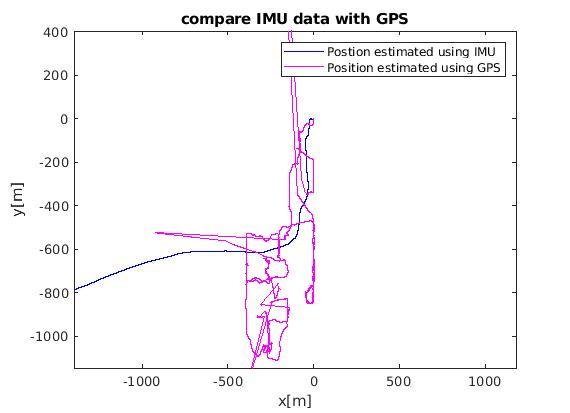
\includegraphics[width = 0.8\linewidth]{media/original-compare.jpg}
    \caption{\textit{Compare IMU data with GPS data.}}
    \label{fig:IMU-GPS}
\end{figure}

\begin{figure}[hbt!]
    \centering
    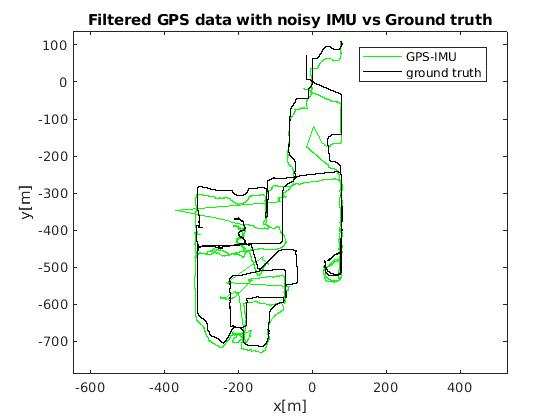
\includegraphics[width = 0.8\linewidth]{media/filteredfGPS.jpg}
    \caption{\textit{GPS data filted by IMU data.}}
    \label{fig:filteredgps}
\end{figure}